% !TeX root = ../../protocolo.tex

Optical metasurfaces are bidimensional arrays of metallic/dielectric nanostructures ---known as meta-atoms--- specifically tailored to behave in a way no found in nature when illuminated at specific wavelengths \cite{khan_optical_2022,gonzalez-alcalde_large_2020}. Depending on the physical properties of the meta-atoms, that is, their composition, size, shape, orientation and distribution within the bidimensional array \cite{kim_plasmonic_2019,khan_optical_2022}, metasurfaces allow to shape at will the  spatial optical response of the system \cite{chen_review_2016}, thus suiting them for a variety of applications in fields such as spectroscopy \cite{khan_optical_2022}, color structuration \cite{gonzalez-alcalde_large_2020}, communications \cite{chen_review_2016}, and sensing \cite{estevez_trends_2014,jain_noble_2008,khan_optical_2022,chen_review_2016,kim_plasmonic_2019}. In the last decades, the interest in optical metasurfaces for medical applications has increased due to  the need for sensitive, fast, low-cost and easy-to-use technologies \cite{estevez_trends_2014,kim_plasmonic_2019}, like metasurfaces with plasmonic (metallic) meta-atoms used as contrasting agents for bioimaging  \cite{kim_plasmonic_2019}, and as free-label biosensors returning real-time measurements \cite{estevez_trends_2014,kabashin_plasmonic_2009,khan_optical_2022}.

Metasurfaces designed for biosensing typically consist of a nanostructurated substrate with compatible microfluidic devices illuminated with a white light source and a light recollection system, allowing for scattering or extinction measurements, followed by an spectrometer \cite{estevez_trends_2014,feuz_improving_2010}. One particular kind of  biosensing-aimed metasurfaces consists in plasmonic meta-atoms, exploiting their property of high confinement of light at nanometric scales, yielding an improvement in the sensitivity of various detection techniques \cite{khan_optical_2022}. The light confinement is the result of the meta-atom's Localized Surface Plasmon Resonances (LSPRs) being excited at the meta-atom's interface with its surroundings, which occurs when the electromagnetic fields couple to the free electrons of the plasmonic structure \cite{chen_review_2016,kim_plasmonic_2019,estevez_trends_2014}.  Since the LSPR is material and geometry dependent, a variety of plasmonic metasurfaces have been designed \cite{feuz_improving_2010,kabashin_plasmonic_2009,qiu_dual_2020,svedendahl_refractometric_2014} ---each with its own benefits and disadvantages \cite{chen_review_2016,estevez_trends_2014}--- as those shown in  Fig. \ref{fig:Back}, all of which are plasmonic metasurfaces consisting of gold (Au) meta-atoms on a glass substrate but with different geometries and distributions within the metasurface.  For example, Feuz et al. \cite{feuz_improving_2010} employed a short-range ordered metasurface of nanoholes to sense protein binding events in real-time [Fig. \ref{sfig:back:a}], while  Kabashin et al. \cite{kabashin_plasmonic_2009} measured  changes in the refractive index of the media embedding an ordered metasurface of plasmonic nanorods [Fig. \ref{sfig:back:b}].  Metasurfaces with simpler geometries and distributions can be used  for biosensing as well, as shown by Qiu et al. \cite{qiu_dual_2020}, who employed a disordered metasurface of nanospheres to detect selected DNA sequences from Severe Acute Respiratory Syndrome Coronavirus 2 (SARS-CoV-2) [Fig. \ref{sfig:back:c}], or by Svedendahl et al. \cite{svedendahl_refractometric_2014}, who sensed protein binding events with a short-range ordered metasurface of nanospheres [Fig. \ref{sfig:back:d}].

\begin{figure}[h!]
\centering
\hspace*{-3.5em}%
\begin{tikzpicture}[scale = .9]
	  \node at (0,0) {  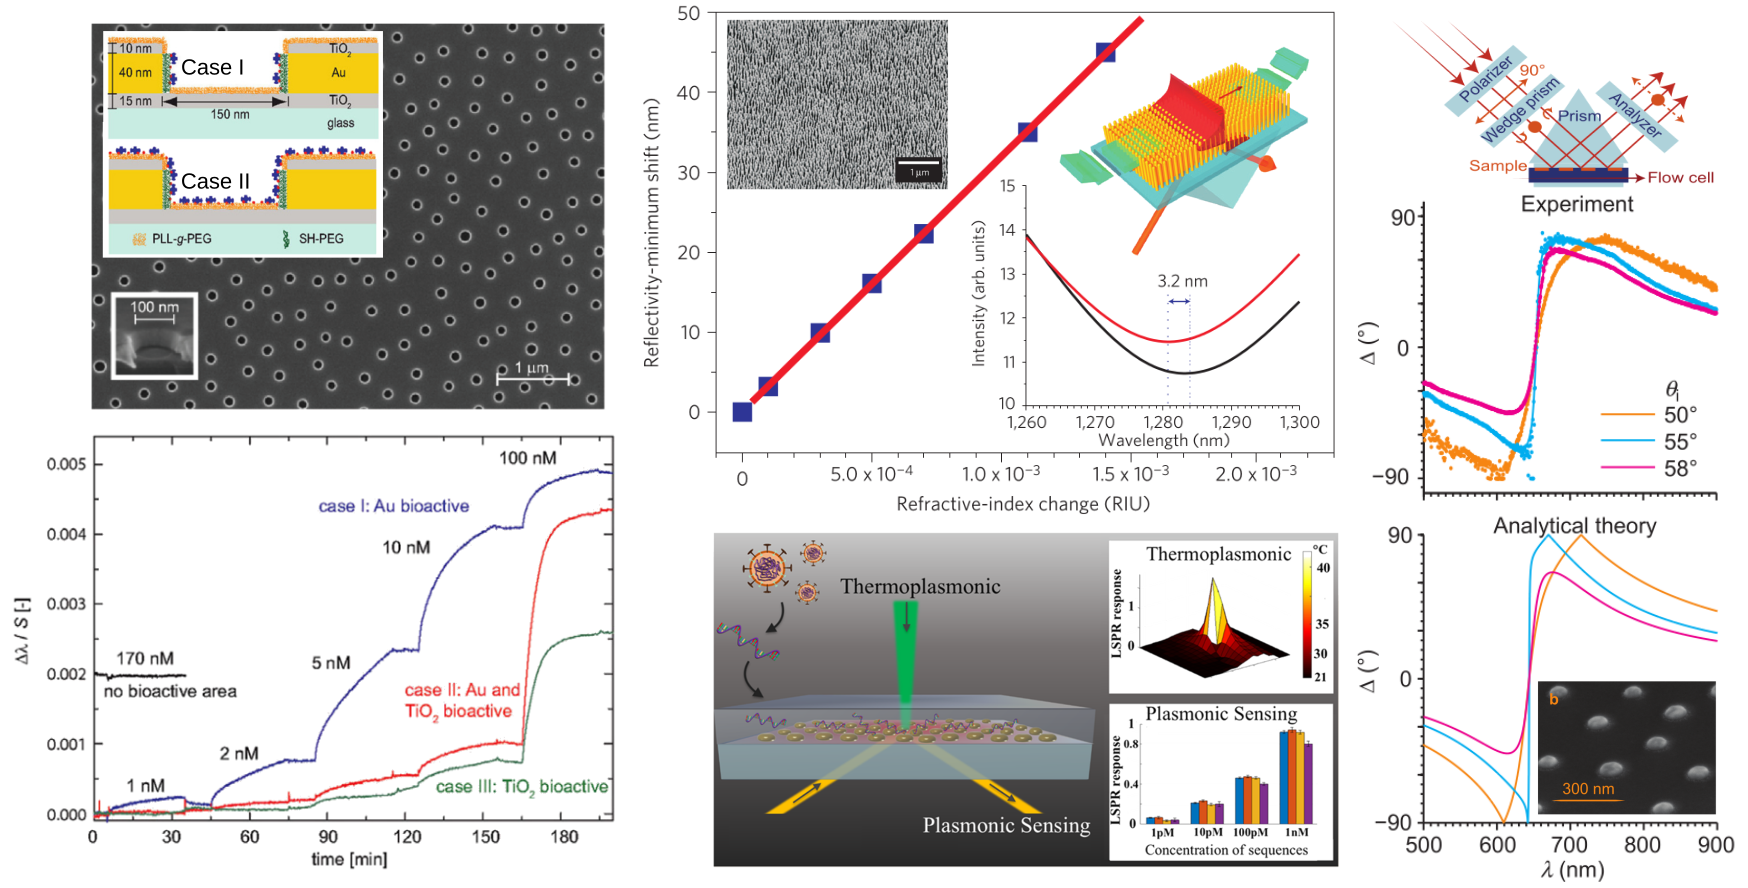
\includegraphics[width = \textwidth]{background.png}};
		\node at (-8.3,4.15) {  \begin{subfigure}{.2\textwidth}\caption{ }\label{sfig:back:a}\end{subfigure}};
		\node at (-2.3,4.15) {  \begin{subfigure}{.2\textwidth}\caption{ }\label{sfig:back:b}\end{subfigure}};
		\node at (-2.3,-1) {  \begin{subfigure}{.2\textwidth}\caption{ }\label{sfig:back:c}\end{subfigure}};
		\node at (5.2,4.15) {  \begin{subfigure}{.2\textwidth}\caption{ }\label{sfig:back:d}\end{subfigure}};
\end{tikzpicture}
  \vspace*{-1.75em}
  \caption[Backgrounds]{Examples of biosensing-aimed plasmonic metasurfaces. \textbf{a)} Short-range ordered metasurface of nanoholes in a Au film [Scanning Electron Microscopy (SEM) image and meta-atom scheme] and real-time measurements of the LSPR redshift due to protein binding events; images extracted and adapted from \cite{feuz_improving_2010}. \textbf{b) } Reflectivity minimum shift of an ordered metasurface of Au nanorods (SEM image and scheme in the inset) as a function of the refractive index change of the media embedding the metasurface; images extracted and adapted from \cite{kabashin_plasmonic_2009}. \textbf{c)} Schematics of a disordered metasurface of Au nanospheres designed for SARS-CoV-2 detection and the LSPR response of its meta-atom: Thermoplasmonic and plasmonic sensing; image extracted from \cite{qiu_dual_2020}. \textbf{d)} Experimental and theoretical results for the ellipsometric parameter $\Delta$ as a function of the incident wavelength, when a short-ranged ordered metasurface of Au nanospheres (SEM image) is illuminated by a  non-polarized white light as shown in the setup diagram; extracted and adapted from \cite{svedendahl_refractometric_2014}.
  }
\label{fig:Back}
\end{figure}

% The design of plasmonic metasurfaces is determined through two main characteristics: its fabrication process and its theoretical behavior. On the one hand, the fabrication process relies on a variety of methods depending on the desired meta-atom's physical properties and distribution. For example, metasurfaces suited for biosensing are commonly  fabricated by lithography techniques, like electron beam lithography (ordered array) or hole-mask colloidal lithography  (ordered and disordered arrays) \cite{estevez_trends_2014}, thermal annealing of thin metallic films (disordered arrays) by dewetting \cite{qiu_dual_2020} or laser ablation \cite{meng_anisotropic_2015}, and chemical growth-methods \cite{estevez_trends_2014,kabashin_plasmonic_2009}. On the other hand, the theoretical behavior estimates the optical response of the metasurface either by numerical methods, like the Finite Element Method (FEM) \cite{feuz_improving_2010}, the Finite Differences Time Domain (FDTD) \cite{qiu_differential_2015}, and the Discrete Dipole Approximation (DDA) \cite{meng_anisotropic_2015}, or by analytical models, like the Thin Island Theory \cite{svedendahl_refractometric_2014,bedeaux_optical_2004}, the Dipolar Model \cite{barrera1991optical} ---both developed for disordered bidimensional arrays of nanospheres on a substrate--- or the Maxwell Garnett Model ---originally developed for 3D colloidal systems of spheres \cite{sihvola_electromagnetic_2008}--- modified to describe bidimensional systems of non-spherical meta-atoms \cite{oates_characterization_2011,kabashin_plasmonic_2009,moirangthem_enhanced_2012}. The study of the theoretical behavior of a metasurface may narrow the desired physical characteristics of the meta-atoms thus directly impacting the choice of the best suited fabrication process and its parameters, however it is stressed that such calculations return the optical response of the metasurface under ideal conditions as, for example, perfect geometrical shapes of the meta-atoms, perfect periodicity or even perfect deposition on the substrate supporting the meta-atoms.

Since LSPRs are excited at frequencies that depend on the material and geometry of the nanostructures, metasurfaces of various configurations have been designed \cite{feuz_improving_2010,kabashin_plasmonic_2009,qiu_dual_2020,svedendahl_refractometric_2014,chen_review_2016,estevez_trends_2014}, as shown in Fig. \ref{fig:ejemplos}. For example, Kabashin et al. \cite{kabashin_plasmonic_2009} reported a biosensing metasurface consisting of cylindrical gold nanoparticles (AuNPs) arranged in a square lattice [see Fig. \ref{fig:Kabashin}]; this metasurface exhibited appropriate sensitivities for detecting changes in the refractive index of aqueous samples. Another example of the versatility and advantages of plasmonic metasurfaces for biosensing is a disordered array of spherical AuNPs on a glass substrate, used by Svedendahl et al. \cite{svedendahl_refractometric_2014} [see Fig. \ref{fig:Svedendahl}] and Qiu et al. \cite{qiu_dual_2020} [see Fig. \ref{fig:Qiu}], who detected real-time protein binding events and SARS-CoV-2 DNA sequences, respectively, by illuminating the metasurface in an internal incidence configuration and measuring the ellipsometric parameters \cite{svedendahl_refractometric_2014,qiu_dual_2020}. It is worth noting that with a random distribution of NPs, fabrication processes such as laser ablation \cite{hammad_improving_2023} or thermal treatment known as \textit{dewetting} \cite{wang_formation_2011,cuanalo_sensitivity_2022} can be employed, reducing fabrication time and cost.

Metasurface design can be achieved using both analytical and numerical methods to estimate the physical characteristics that optimize their optical response for a given application. For example, the resonance wavelengths of LSPRs in ordered metasurfaces of arbitrary nanostructures have been calculated using the Finite Element Method (FEM) \cite{feuz_improving_2010} or the Finite-Difference Time-Domain (FDTD) algorithm \cite{qiu_differential_2015}. Additionally, the optical response of disordered metasurfaces of spherical NPs has been analytically studied using effective medium theories under the small-particle approximation \cite{reyes2022enhancement}. These models describe two-dimensional arrays as equivalent continuous media \cite{bosi_transmission_1992}.


 The motivation for such a physical system arises from the collaboration between two experimental research groups\footnote{The Biophotonics Group and the Organic and Hybrid Semiconductor Optoelectronics Group at \textit{Instituto Nacional de Astronomía, Óptica y Electrónica} (INAOE).} and one theoretical research group\footnote{The Nanoplasmonics Group at \textit{Facultad de Ciencias, Universidad Nacional Autónoma de México} (UNAM).}. The experimental groups have fabricated disordered arrays of partially embeded Au nanospheres with an average radius of $12.5$ nm ---a potential meta-atom for biosensing-aimed metasurfaces---. 

 During the design stage of metasurfaces, both analytical and numerical methods can be employed to estimate the physical characteristics that optimize their optical response based on the intended application. For instance, the wavelengths at which LSPRs of ordered metasurfaces composed of arbitrary nanostructures are excited have been calculated using the Finite Element Method (FEM) \cite{feuz_improving_2010} or the Finite-Difference Time-Domain (FDTD) algorithm \cite{qiu_differential_2015}. Likewise, the optical response of disordered metasurfaces consisting of spherical NPs has been analytically studied using the effective medium theories under the small-particle approximation \cite{reyes2022enhancement}, where the response of two-dimensional arrays is modeled as an equivalent continuous medium \cite{bosi_transmission_1992}. Examples of effective medium theories include the Dipolar Model (DM) \cite{barrera1991optical,reyes2022enhancement}, the Island Film Theory (IFT) \cite{bedeaux_optical_2004,svedendahl_fano_2012,svedendahl_refractometric_2014}, and modifications to the Maxwell Garnett Model \cite{kabashin_plasmonic_2009}.

The characterization of a metasurface involves determining its physical properties, such as geometry, material composition, and spatial distribution of its nanostructures. One way to perform characterization is through imaging techniques such as Transmission Electron Microscopy (TEM), Scanning Electron Microscopy (SEM), and Atomic Force Microscopy (AFM). However, these methods often lead to sample damage or partial destruction. An alternative to these invasive methods is to compare optical measurements with theoretical results—obtained through numerical or analytical calculations—so that the calculated response matches the experimental data for specific metasurface parameters. For example, since the spectral position of the LSPR depends on the geometry and size of an NP, it can be identified by comparing reflectance measurements with estimated values. It is important to note that this approach requires the theoretical conditions to be reproducible in a laboratory setting.

In the case of disordered metasurfaces, effective medium theories such as DM or IFT are suitable for describing the optical response of metasurfaces composed of spherical NPs—small relative to the wavelength of illumination—perfectly positioned on a dielectric substrate \cite{barrera1991optical,bedeaux_optical_2004}. Both DM and IFT describe each spherical NP in the two-dimensional array as an electric dipole, allowing for relaxation of the perfect spherical geometry assumption by introducing depolarization factors, thereby extending these models to ellipsoids \cite{sihvola_electromagnetic_2008}. Additionally, DM and IFT can be applied without modification even if partial embedding of the NPs into the substrate is identified, as long as it does not exceed 12\% of the NP's volume\footnote{In my master's thesis, FEM calculations of absorption and extinction cross-sections of a 12.5 nm radius AuNP illuminated in the visible spectrum showed that the LSPR shift relative to the case of a perfectly positioned NP was at most 5 nm when the embedding depth was one-eighth of its volume.}. Although certain geometric and embedding conditions can be relaxed while still accurately describing the behavior of disordered metasurfaces, this does not apply to all assumptions of DM or IFT, such as modeling all NPs as electric dipoles.

Both DM and IFT require the small-particle approximation, meaning a disordered metasurface of spherical NPs must have a narrow size distribution. However, if NP synthesis is performed using physical methods such as laser ablation or \textit{dewetting}, the size distribution may exhibit a normal distribution with significant standard deviation \cite{hammad_improving_2023} or a log-normal distribution \cite{wang_formation_2011,vazquez-estrada_optical_2014}, as illustrated in Fig. \ref{fig:dist}. In such cases, some NPs within the metasurface may be large enough to require higher-order multipolar contributions beyond the dipolar approximation to accurately describe their optical response. When the small-particle approximation does not hold for a real sample, scattering theories can be used, which do not require the small-particle approximation and, unlike effective medium theories, do not describe the metasurface as an equivalent continuous film but rather provide an approximate solution to Maxwell's equations \cite{bosi_transmission_1992,reyes2018analytical}. A scattering theory that describes disordered arrays of spherical NPs with a given size distribution is the Coherent Scattering Model, which can be used to design and characterize metasurfaces of spherical NPs under more realistic experimental conditions. The following section presents the hypotheses, characteristics, and expressions of this model.
